\documentclass[10pt, a4paper]{article}
\usepackage[latin1]{inputenc}
\usepackage{amsmath}
\usepackage{amsfonts}
\usepackage{amssymb}
\usepackage{graphicx}
\usepackage{xcolor}
\usepackage{float}
\usepackage{hyperref}
\usepackage{booktabs}
\usepackage[normalem]{ulem}
\usepackage{cite}

\usepackage{xcolor}
\hypersetup{
    colorlinks,
    linkcolor={red!50!black},
    citecolor={blue!50!black},
    urlcolor={blue!80!black}
}

% Forcequit autonumbering
\pagenumbering{gobble}


%% Multicolumns
\usepackage{multicol}
\setlength{\columnsep}{1cm}


% Margin to left and middle
\usepackage[margin={2cm,1cm}]{geometry}


\title{Immaterialist Fashion - Report}

\author{Mick van Hulst \and Dennis Verheijden \and Roel van der burg \and Brian Westerweel \and Joost Besseling}

\begin{document}
	\maketitle
	
	
	%% Start multicolumns
	\begin{multicols}{2}
	
	    \section{Introduction}
	    This report describes the results for the first competition of the course Machine Learning in Practice. The source code for this project can be found by going to \href{https://github.com/mickvanhulst/imaterialist_kaggle}{the public Github repository}.
	    \\
	    \\
	    During the project each of the team members were assigned specific tasks. Do take note that our approach can be considered agile as we switched roles constantly and helped each other out where we could:
	    \begin{itemize}
	        \item \textbf{Mick van Hulst:} Exploratory data analysis, GCP, Batch generator, implementing ResNet
	        \item \textbf{Dennis Verheijen:} Implementing networks, general code cleaning, weight determination
	        \item \textbf{Roel van der Burg:} Exploratory data analysis, implementing ResNet
	        \item \textbf{Brian Westerweel:} Implementing custom F1-measure, Object-detection, Report
	        \item \textbf{Joost Besseling:} Object-detection, Ensemble algorithm
	    \end{itemize}
		
		\section{Problem statement}
		We have chosen \href{https://www.kaggle.com/c/imaterialist-challenge-fashion-2018}{the immaterialist fashion challenge} on Kaggle. This challenge consisted of a data set of approximately 1.1 million images which had to be assigned one or multiple labels. In total there are 228 labels that could be assigned of which most don't make sense for the human mind.
		
		
		\section{Data set}
		Kaggle provided a training, validation and test set, combined they consist of approximately 1.1 million images. For each image there is a list containing one or more labels. As mentioned earlier for most of the labels it is unclear why images have a certain label (figure \ref{fig:label_24_examples}). 
		\\
		\begin{figure}[H]
            \centering
            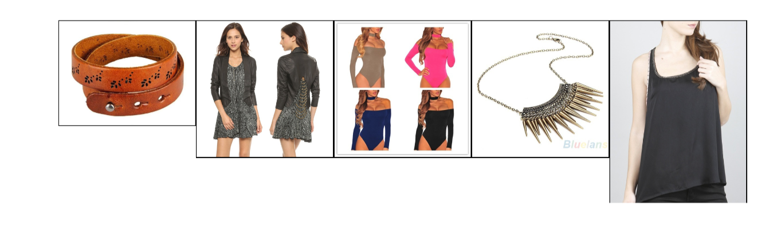
\includegraphics[scale=.4]{img/label24_examples.png}
            \caption{Example images for label 24.}
            \label{fig:label_24_examples}
        \end{figure}
        
        When looking at the individual images label 24 could either be a shirt, necklace, skirt or bracelet. However, apparently there is a more general feature in this images that is represented by label 24 which we couldn't think of.
		
		Another important characteristic of this data set is that it is quite imbalanced (figure \ref{fig:data_dist}). There are around 20 labels which occur more than a 100.000 times each while most of the other labels have roughly 30.000 occurrences.
		\\
		\begin{figure}[H]
            \centering
            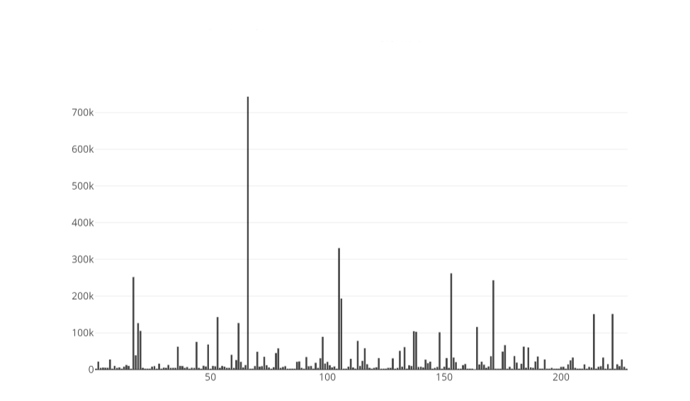
\includegraphics[scale=.4]{img/data_distribution.png}
            \caption{Data distribution, each value on the x-axis representing the label and on the y-axis are the occurences for the labels.}
            \label{fig:data_dist}
        \end{figure}
        The imbalance in the data set posed the challenge of properly training our network by making sure that it doesn't label all images with the most occurring label. This can, for example, be done by setting weights to the different classes so incorrectly labeling a rare label is more heavily penalized than incorrectly labeling a very common label.
	
		\subsection*{Data Preprocessing}
		The data for this challenge didn't need a lot of sanitizing. However, the images were of different sizes and because convolutional neural networks need a static input size we needed to make sure that all images that were fed to the network had the same size. This is accomplished by implementing a patch generator that cut same-sized patches from the source images. 
		
		It has to be noted that due to the gigantic disc size that was needed for the data we decided to download the images at 85\% of the available quality.
		
		\section{Models}
		In contrast to the last project we decided to use pre-trained model for this challenge, instead of fully training the models ourselves. 
		
		The models used in this project are pre-trained using ImageNet \cite{deng2009imagenet}. ImageNet is a collection of over 100.000 concepts with average 1000 images per concept. Also, ImageNet is often used as a reference data set for setting convolutional neural network benchmarks.
		
		For this project MobileNet, InceptionV3, Xception and ResNet50 are chosen because these model individually have a good performance for image classification problems. Therefore, we think that combining the models with ensemble learning methods will yield even better results. Besides the well-known models we created a model based on object detection.
		
		In this way we ensure that the data knows all the possible labels it has to predict and the relation between the target data and the labels. By using the pre-trained weights for the different models they are already aware of the high-level abstraction for images. These abstractions have proven to work well on image classification tasks \cite{razavian2014cnn}.
		For fine-tuning the different models the last layers of each models are unfrozen. Unfreezing the last layers make it possible to train them on another data set. These partly unfrozen models are trained on the training data from the challenge.
		
		Because the data was imbalanced to train the models on three data sets. The first one consists of all available training data. The other two data sets are mutually exclusive subsets of the total data set. One contains only the labels that occur more than 100.000 times, while the other contains the labels that have less than 100.000 occurrences.
		
		For the loss of all models binary cross entropy is used, because the model has to output a probability for each label. To measure performance of the models a micro-averaged F1-score is used, because this also is the performance metric used by Kaggle. Hyper parameters are left as they were implemented by Keras.
		
		\subsection{Object detection}
		For the object detection model we first predicted objects for each image using a pre-trained ResNet50 \cite{DBLP:journals/corr/HeZRS15} trained on the open image data set \cite{openimages}. For each image we used the found objects as features for that image and used those features to train another neural network. 
		
		However, because the object detection network very often detected just a few objects. Because the object detection network resulted in very small features per image we found very early on that this network would not yield any noteworthy results. Therefore, this model has not been further developed.
		
		\subsection{ResNet50}
		The ResNet we used is based on Keras' version \cite{DBLP:journals/corr/HeZRS15}, where the last layer was unfrozen and fine-tuned to our target data set. 
		
		TODO: MORE EXPLANATION + RESULTS, ROEL HAS SUMBISSION
		
		\subsection{MobileNet}
		MobileNet again is based on a version of Keras \cite{howard2017mobilenets}. In this case the last 5 layers are unfrozen and trained on the training images of this challenge.
		
		TODO: MORE EXPLANATION + RESULTS, NOT SUBMITTED (At least with thresholds)
		
		\subsection{InceptionV3}
		The InceptionV3 \cite{DBLP:journals/corr/SzegedyVISW15} is a convolutional neural network developed by Google. Inception has a very big difference with other conventional neural networks because of how their layers are build.
		
		In most convolutional networks a decision has to be made for each layer in which you can either do 5x5, 3x3 or 1x1 convolutions, max-pooling. Inception refuses to make the choice for one layer above the other and decided to do everything within one layer. This architecture makes the network very time expensive to train because it is basically brute-forcing the different options that are available.
		
		TODO: RESULTS
		
		\subsection{Xception}
		
		
		\section{Thresholding}
		
		TODO: HOW DID WE THRESHOLD
		
		\section{Ensembling}
		
		The data set is highly imbalanced. To counteract this we decided to train two special classifiers. The first classifier is only trained on the labels that occur at least 100 000 times. The other classifier is trained on the remaining labels. These two classifier are combined into one classifier, by simply . The imbalance for both classifiers is lower than the imbalance for the total data set. 

        We also trained multiple networks on all labels. We now want to combine these networks to give a single prediction on the test set. We will ensemble them with weighted soft voting. 

        To calculate the weights we generate the predictions for the validation set, and then use an optimization algorithm to find the optimal weights on this set. We have implemented a simple hill climbing algorithm and also PSO (Particle Swarm Optimization) to calculate the weights. 

        An interesting side effect of using this weighting algorithm is that we find which models work well, and which models don't work as well. 

        Results for:

        simple average
        hill climbing
        pso
        harmonic mean

        We can see that the results of the PSO algorithm are the most convincing. If we look at the weights that are generated by this strategy, we can see that the combined classifier is relatively important. This validates our idea that we could counteract the imbalance by training two seperate classifiers.


        TODO: make a nice table of the ensembling results. And say something about these results.
		
		\section{Conclusion}
		
		TODO: WHAT CAN WE SAY?
	
		\section{Reflection}
		This section briefly discusses some things that stood out during this project.
	    
	\bibliographystyle{unsrt}
	\bibliography{bib}
	\end{multicols}
	
\end{document}